\documentclass[12pt, a4paper]{report}
\usepackage[utf8]{inputenc}

\usepackage[T1]{fontenc}
\usepackage[english, french]{babel}
\usepackage{graphicx}
\usepackage{fullpage}
\usepackage{eso-pic}
\usepackage{tcolorbox}
\usepackage{hyperref}
\usepackage[toc]{glossaries}
\usepackage{tikz}

\usepackage{listings}
\usepackage{background}
\usepackage{setspace}
\usepackage{titlepic}

\usepackage{hyperref}
\usepackage{natbib}

% Définir les paramètres de l'image de fond pour la première page
\backgroundsetup{
	scale=2.5, % Échelle de l'image
	color=black, % Couleur de l'image (noir et blanc par défaut)
	opacity=0.1, % Opacité de l'image
	angle=0, % Angle de rotation de l'image
	position=current page.center, % Position de l'image centrée
	vshift=0cm, % Décalage vertical
	hshift=0cm, % Décalage horizontal
	contents={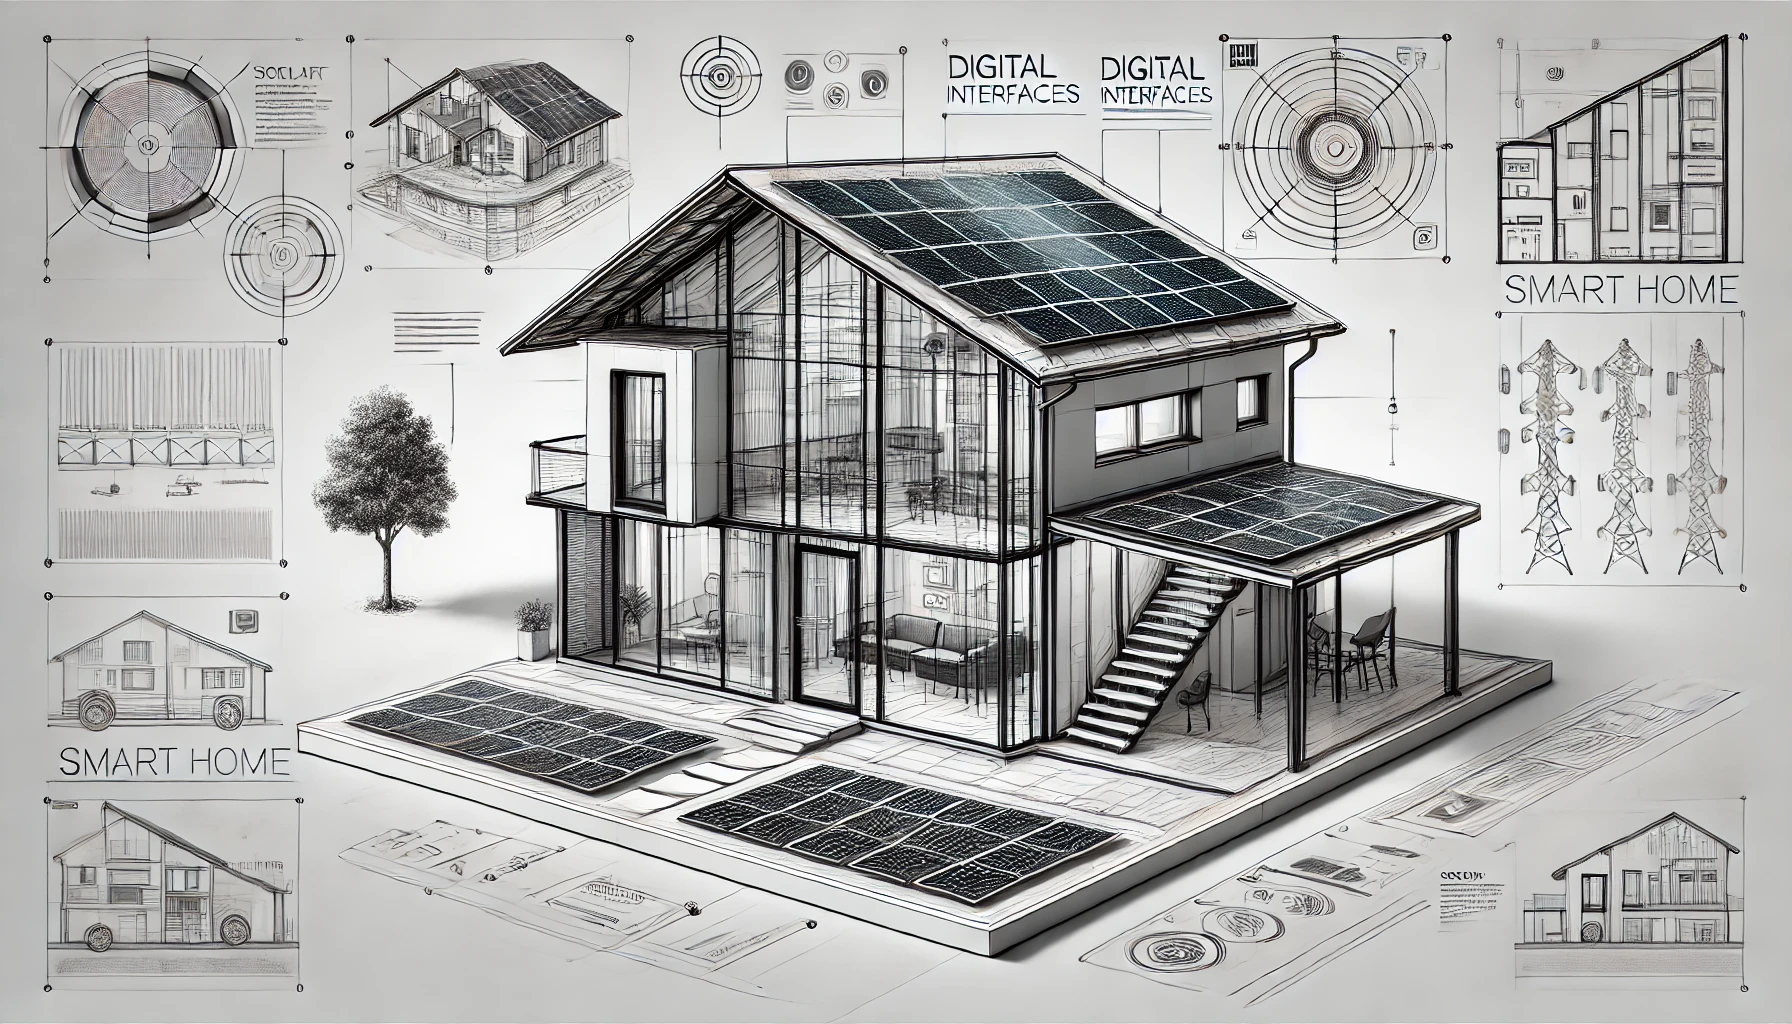
\includegraphics[width=\paperwidth]{ressources/img/logos/imageSmartHouse}} % Contenu (image de fond)
}

\usepackage[a4paper, top=2.5cm, bottom=2.5cm, left=3cm, right=2cm]{geometry}

% Pour la lisibilité, on peut utiliser le package setspace pour ajuster l'espacement entre les lignes
\usepackage{setspace}
\usetikzlibrary{positioning, decorations.pathreplacing}

\definecolor{darkWhite}{rgb}{0.94,0.94,0.94}

\lstset{
	aboveskip=3mm,
	belowskip=-2mm,
	backgroundcolor=\color{darkWhite},
	basicstyle=\footnotesize,
	breakatwhitespace=false,
	breaklines=true,
	captionpos=b,
	commentstyle=\color{red},
	deletekeywords={...},
	escapeinside={\%*}{*)},
	extendedchars=true,
	framexleftmargin=16pt,
	framextopmargin=3pt,
	framexbottommargin=6pt,
	frame=tb,
	keepspaces=true,
	keywordstyle=\color{blue},
	language=Python,
	literate=
	{²}{{\textsuperscript{2}}}1
	{⁴}{{\textsuperscript{4}}}1
	{⁶}{{\textsuperscript{6}}}1
	{⁸}{{\textsuperscript{8}}}1
	{€}{{\euro{}}}1
	{é}{{\'e}}1
	{è}{{\`{e}}}1
	{ê}{{\^{e}}}1
	{ë}{{\¨{e}}}1
	{É}{{\'{E}}}1
	{Ê}{{\^{E}}}1
	{û}{{\^{u}}}1
	{ù}{{\`{u}}}1
	{â}{{\^{a}}}1
	{à}{{\`{a}}}1
	{á}{{\'{a}}}1
	{ã}{{\~{a}}}1
	{Á}{{\'{A}}}1
	{Â}{{\^{A}}}1
	{Ã}{{\~{A}}}1
	{ç}{{\c{c}}}1
	{Ç}{{\c{C}}}1
	{õ}{{\~{o}}}1
	{ó}{{\'{o}}}1
	{ô}{{\^{o}}}1
	{Õ}{{\~{O}}}1
	{Ó}{{\'{O}}}1
	{Ô}{{\^{O}}}1
	{î}{{\^{i}}}1
	{Î}{{\^{I}}}1
	{í}{{\'{i}}}1
	{Í}{{\~{Í}}}1,
	morekeywords={*,...},
	numbers=left,
	numbersep=10pt,
	numberstyle=\tiny\color{black},
	rulecolor=\color{black},
	showspaces=false,
	showstringspaces=false,
	showtabs=false,
	stepnumber=1,
	stringstyle=\color{gray},
	tabsize=4,
	title=\lstname,
}

% Additional language definitions
\lstdefinelanguage{JavaScript}{
	keywords={typeof, new, true, false, catch, function, return, null, catch, switch, var, if, in, while, do, else, case, break},
	keywordstyle=\color{blue}\bfseries,
	ndkeywords={class, export, boolean, throw, implements, import, this},
	ndkeywordstyle=\color{darkgray}\bfseries,
	identifierstyle=\color{black},
	sensitive=false,
	comment=[l]{//},
	morecomment=[s]{/*}{*/},
	commentstyle=\color{purple}\ttfamily,
	stringstyle=\color{orange}\ttfamily,
	morestring=[b]',
	morestring=[b]"
}

\lstdefinelanguage{C}{
	keywords={auto, break, case, const, continue, default, do, double, else, enum, extern, float, for, goto, if, inline, int, long, register, restrict, return, short, signed, sizeof, static, struct, switch, typedef, union, unsigned, void, volatile, while, _Bool, _Complex, _Imaginary},
	keywordstyle=\color{blue}\bfseries,
	identifierstyle=\color{black},
	sensitive=true,
	comment=[l]{//},
	morecomment=[s]{/*}{*/},
	commentstyle=\color{green}\ttfamily,
	stringstyle=\color{red}\ttfamily,
	morestring=[b]',
	morestring=[b]"
}

\makeglossaries
\newglossaryentry{API}
{
	name=API,
	description={(Interface de Programmation d'Application) est un ensemble de protocole permettant à différentes applications logicielle d'echanger des données entre elles}
}

\newcommand{\HRule}{\rule{\linewidth}{0.5mm}}
\newcommand{\blap}[1]{\vbox to 0pt{#1\vss}}
\newcommand\AtUpperLeftCorner[3]{%
	\put(\LenToUnit{#1},\LenToUnit{\dimexpr\paperheight-#2}){\blap{#3}}%
}
\newcommand\AtUpperRightCorner[3]{%
	\put(\LenToUnit{\dimexpr\paperwidth-#1},\LenToUnit{\dimexpr\paperheight-#2}){\blap{\llap{#3}}}%
}

\title{\LARGE{Smarthouse}}
\author{\textsc{Khedhaouria} Eliès \& \textsc{Marcelet} Paul}
\date{\today}
\makeatletter



\begin{document}
	\onehalfspacing % Définit l'espacement entre les lignes à 1.5
	
	
	\begin{titlepage}
		
		
		\enlargethispage{2cm}
		
		\AddToShipoutPicture{
			\AtUpperLeftCorner{1.5cm}{1cm}{
\includegraphics[width=6.5cm]{ressources/img/logos/isimaInp.png}}
		}
		
		\begin{center}
			\vspace*{10cm}
			
			\LARGE{\textbf{Rapport d'élève Ingénieur}}\\
			\LARGE{\textbf{Projet de troisième année}}\\
			\large{Filière:\textbf{ Sécurité} et \textbf{réseaux}} 
			\HRule
			\vspace*{0.5cm}
			\Huge{\textsc{\textbf{\@title}}}\\
			
		\end{center}
		\vspace*{2.5cm}
		Présenté par: \textbf{\@author }
		
		\vspace*{4.5cm}
		Responsable Isima: Monsieur \textbf{Alexandre GUITTON} \hspace*{2cm} Date de soutenance: \textbf{02/07/2024}\\\\
		\textbf{Campus des Cézeaux .  1 rue de la Chébarde .  TSA 60125 .  63178  Aubière CEDEX}
		
		
		
	\end{titlepage}
	\backgroundsetup{contents={}}
	\ClearShipoutPicture
	\newpage
	
	\section*{Remerciements}
	
	\tableofcontents
	\listoffigures
	
	\begin{abstract}
		\selectlanguage{french}
	Dans le cadre de notre \textbf{projet de fin d’études}, nous avons conçu et développé un \textbf{système de maison intelligente} 
	capable de transmettre \textbf{des données en temps réel de manière sécurisée} vers un serveur distant. L’objectif principal est de 
	mettre en place un \textbf{système de monitoring avancé}, permettant à un propriétaire de superviser et d’analyser les données 
	générées par ses équipements connectés.
	
	Pour garantir \textbf{l’intégrité et la confidentialité des échanges}, nous avons implémenté une \textbf{communication sécurisée 
	basée sur des certificats SSL/TLS} et le protocole \textbf{MQTTs}, assurant ainsi une transmission chiffrée et authentifiée entre 
	la maison et le serveur.
	
	Les données collectées par les capteurs sont stockées dans une \textbf{base de données à série temporelle} (InfluxDB), 
	spécialement optimisée pour le traitement et l’analyse de données en flux continu.
	
	Une \textbf{API centralisée}, développée en \textbf{Laravel}, a été mise en place afin de :
	\begin{itemize}
		\item \textbf{Gérer la création des propriétaires} et l’association sécurisée de leurs équipements.
		\item \textbf{Automatiser la génération et la signature des certificats} pour garantir une authentification fiable.
		\item \textbf{Offrir une interface d’accès aux données}, permettant aux utilisateurs de récupérer \textbf{des données en temps 
		réel ou historiques}, selon différents filtres appliqués à la base de données.
	\end{itemize}
	
	Enfin, une \textbf{interface graphique interactive}, développée en \textbf{Qt}, permet aux utilisateurs de \textbf{visualiser les 
	données en temps réel} sous forme de \textbf{graphiques dynamiques}. Cette interface interagit directement avec l’API afin de 
	récupérer et d’afficher \textbf{les données filtrées}, qu’elles soient en temps réel ou issues d’une période spécifique dans le 
	passé.
	
	Ce projet intègre \textbf{des technologies modernes et des concepts avancés en sécurité, IoT, gestion des bases de données et 
	visualisation de données en temps réel}, assurant ainsi une \textbf{infrastructure robuste, fiable et évolutive}.

	\end{abstract}
	\selectlanguage{english}
	\begin{abstract}
		As part of our \textbf{final-year engineering project}, we designed and developed a \textbf{smart home system} capable of 
		securely transmitting \textbf{real-time data} to a remote server. The main objective is to implement an \textbf{advanced 
		monitoring system} that allows a homeowner to monitor and analyze data generated by their connected devices.
		
		To ensure \textbf{data integrity and confidentiality}, we implemented a \textbf{secure communication protocol based on SSL/TLS 
		certificates} and the \textbf{MQTTs protocol}, providing encrypted and authenticated communication between the home and the 
		server.
		
		Sensor data is stored in a \textbf{time-series database} (InfluxDB), optimized for real-time data processing and analysis.
		
		A \textbf{centralized API}, developed in \textbf{Laravel}, has been implemented to:
		\begin{itemize}
			\item \textbf{Manage the creation of homeowners} and the secure association of their devices.
			\item \textbf{Automate the generation and signing of certificates} to ensure reliable authentication.
			\item \textbf{Provide a data access interface}, allowing users to retrieve \textbf{real-time or historical data} based on 
			various filters applied to the database.
		\end{itemize}
		
		Finally, an \textbf{interactive graphical interface}, developed in \textbf{Qt}, allows users to \textbf{visualize real-time 
		data} using \textbf{dynamic graphs}. This interface directly interacts with the API to retrieve and display \textbf{filtered 
		data}, whether in real-time or from a specific historical period.
		
		This project integrates \textbf{modern technologies and advanced concepts in security, IoT, database management, and real-time 
		data visualization}, ensuring a \textbf{robust, reliable, and scalable infrastructure}.
		
	\end{abstract}
	
	
	\chapter{Introduction}
		La \textbf{domotique} représente aujourd'hui un enjeu majeur dans le domaine des innovations technologiques. Avec l'essor des 
		\textbf{maisons connectées} et des \textbf{IOTs}, les utilisateurs peuvent désormais \textbf{surveiller} et \textbf{contrôler} 
		leur domicile à distance, leur assurant ainsi une amélioration significative en termes de \textbf{sécurité}, 
		\textbf{d'efficacité énérgétique} et de \textbf{confort}. Cette évolution s'inscrit dans un contexte plus large dans lequel 
		l'automatisation et la connectivité jouent un rôle crucial dans notre quotidien.\\
		Le \textbf{monitoring à distance} des équipements d'une maison constitue un axe fondamental de la domotique moderne. Il permet 
		aux propriétaires d'obtenir une \textbf{vue globale de l'état de leur habitation en temps réel}. Cela joue un rôle crucial dans 
		plusieurs domaines:\\
		\begin{itemize}
			\item Il permet de \textbf{sécuriser} un domicile, permettant par exemple la détéction d'intrusion ainsi que la prévention 
			des cambriolages
			
			\item Il permet également une \textbf{optimisation énérgétique} du domicile, par le biais de l'automatisation des objets 
			connectés, en fonction d'horraires programmés, afin d'optimiser la consommation d'énergie.
			
			\item Il permet enfin \textbf{un confort et un contrôle à distance}, offrant aux propriétaires la possibilité d'activer ou 
			de désactiver certains dispositifs sans être physiquement présent.
		\end{itemize}
		Si ces avancées technologiques offrent des opportunités considérables, elles soulèvent néanmoins une problématique critique: 
		\textbf{la sécurisation des dispositifs IoTs et du transfert des données}. Aujourd'hui, de nombreux objets connectés sont 
		déployés avec des failles de sécurité importantes souvent négligées par les fabricants et les utilisateurs. Des outils comme 
		\textbf{Shodan}, un moteur de recherche spécialisé dans l'identification des appareils connectés exposés sur Internet, mettent 
		en évidence la vulnérabilité de nombreux systèmes IoTs accessibles sans protection adéquate. Cette situation constitue un risque 
		majeur, rendant possible des cyberattaques capables de compromettre \textbf{l'intégrité} et \textbf{la confidentialité} des 
		données échangées.\\
		Ce rapport décrit une architecture, solution à cette problématique en explorant l'une des applications majeures de la domotique: 
		\textbf{le monitoring à distance des capteurs d'une maison connectée, ainsi que l'établissement d'une communication sécurisée et 
		authentifiée entre celle-ci et un serveur distant}. L'objectif est de permettre aux utilisateurs de récupérer des \textbf{données 
		en temps réel}, issues de capteurs de leur domicile tout en garantissant \textbf{une transmission chiffrée} afin de protéger les 
		échanges contre d'éventuelles interceptions malveillantes. C'est à partir de cela que l'on peut définir une problématique à 
		laquelle la solution doit répondre: \textbf{Comment développer un système de monitoring en temps réel pour une maison connectée, 
		garantissant la sécurité de la transmission des données tout en renforcant l'authentification des équipements IoTs ?}
		
	
	\chapter{Contexte du Projet}
	\section{Analyse du besoin et définition des objectifs}
		Lorsqu'un résident quitte son domicile, il peut être préoccupé par l'état de sa maison, se demandant si une lumière a été éteinte ou si une fenêtre a été correctement fermée. Ces préoccupations sont légitimes, d'autant plus les statistiques récentes indiquent une augmentation des cambriolages de logements en France. En effet au 30 juin 2024, les forces de sécurité ont enregistré une hausse de 4\% des cambriolages de logements sur les douze derniers mois\footnote{source: \url{https://www.interieur.gouv.fr/actualites/actualites-du-ministere/analyse-conjoncturelle-des-crimes-et-delits-enregistres-par} et \url{https://mobile.interieur.gouv.fr/Interstats/Actualites/Info-Rapide-n-43-La-delinquance-enregistree-par-la-police-et-la-gendarmerie-nationales-un-point-a-mi-annee-2024}}. Cette tendance souligne la nécessité de renforcer les dispositifs de sécurité pour protéger les habitations.\\
		Parallèlement, la proliférations des dispositifs IOT dans les foyers pose des défis non négligeables en matière de cybersécurité. Bien que ces technologies offrent des avantages indéniables en termes de confort et d'efficacité énergetiques, elles peuvent constituées des points d'entrée pour les cybercriminelles si elle ne sont pas correctement sécurisées. Il est ainsi essentiel de garantir que seuls les propriétaires autorisés aient accès à ces dispositifs et que les données transmises soient protégés contre toute altération ou interception malveillante.\\
		Fâce à ces constats, notre projet vise à développer une solution permettant la transimission sécurisée issues de capteurs IoT d'une maison vers un serveur distant. Cette solution devra assurer l'authentification des dispositifs, garantir l'intégrité ainsi que la confidentialité des données, et ainsi permettre aux propriétaires de surveiller à distance l'état de leur domicile en temps réel.
	\section{Organisation de la conception à la création}
	Dans le cadre du développement de ce projet, nous avons adopté une approche structurée en plusieurs phases allant de la simulation initiale de l'environnement domotique jusqu'à la mise en place d'une infrastructure de communication sécurisée et fiable.\\\\
	\textbf{Phase 1: Simulation de l'environnement domotique et émission des données}\\
	Avant de mettre en place l'architecture réseau et serveur, nous avons débuté par la simulation logicielle de la maison connectée, en programmant un environnement permettant la génération de données de divers capteurs (température, humidité, lumière...). Cette simulation développée en \textbf{Python},modélise une maison contenant divers équipements Iots et capteurs emettant des séries de données à temps réel.\\
	L'objectif principal de cette étape était de tester l'envoie de séries de données, à intervalle régulier, au sein d'un serveur distant (Phase suivante), en utilisant le protocole de communication \textbf{MQTT}. A ce moment là, la transmission s'effectuait sans authentification ni chiffrement, nous permettant ainsi, de valider l'intégralité du transport, la récéption au serveur et d'évaluer aussi les performances du protocole. \\\\
	\textbf{Phase 2: Mise en place de l'infrastructure serveur}\\
	Une fois la simulation fonctionnelle, nous avons déployé une \textbf{infrastructure serveur} sous une machine virtuelle \textbf{Ubuntu}, utilisant l'hyperviseur \textbf{Virtualbox} avec un accès par pont en configuration réseau. Ce serveur assure le rôle de récépteur des données envoyées par la maison connectée.\\
	Afin de permettre la récéption ainsi que le sotckage des données, nous avons mit en place plusieurs composants essentiels:\\
	\begin{itemize}
		\item \textbf{Mosquitto}: Un broker \textbf{MQTT} permettant la gestion des messages entres les maisons connectées et le serveur aux divers topics.
		\item \textbf{InfluxDB}: Une \textbf{base de données à séries temporelles}, choisie pour sa capacité à stocker et traiter efficacement des flux de données en temps réel.
		\item \textbf{Telegraf}: Un agent de collecte des données utilisé pour formaliser et structure les données recues depuis le \textbf{Broker} avant leur insertion dans la base de données.
	\end{itemize}
	À la fin de cette étape, après configuration des composantes, l’infrastructure était fonctionnelle, mais vulnérable : les données envoyées par les capteurs n’étaient pas protégées et n’importe quel utilisateur pouvait intercepter ou publier des messages MQTT sur le serveur, compromettant ainsi l’intégrité du système.\\\\
	\textbf{Phase 3: Sécurisation des échanges et authentifications des Maisons}\\
	Afin de garantir l'\textbf{authenticité des émetteurs} et de protéger les données échangées, nous avons implémenté une \textbf{authentification basée sur des certificats SSL/TLS} pour le protocole MQTT. Cette sécurisation repose sur \textbf{l'utilisation de certificats clients} généré par une autorité de certifcation interne au serveur, l'exigence d'une \textbf{authentification mutuelle} entre la maison et le serveur pour toute communication MQTT ainsi que le \textbf{chiffrement des échanges} grâce à TLS emêchant toute interception des données transmises.\\
	Ce mécanisme permet ainsi de \textbf{garantir l'identité des dispositifs connectés} et d'empêcher ainsi toute inteception des données par un acteur non autorisé.\\\\
	\textbf{Phase 4 : Développement d’une API centralisant l’accès aux données}\\
	Afin de faciliter l'accès aux données, d'éviter une exposition directe du broker MQTT et aussi de permettre par la suite la création d'interfaces fonctionnant sur divers plateformes, nous avons développé une \textbf{API Rest sous laravel}, jouant deux rôles importants:\\
	\begin{itemize}
		\item \textbf{Gestion de propriétaires et authentification:} L'API permet la \textbf{création de propriétaires} assurant une authentification unique et sécurisée. Un nouvel utilisateur peut en effet s'enregistrer en tant que propriétaire, l'API lui générera ainsi un \textbf{token unique}, qui servira \textbf{d'identifiant primaire} pour toutes les interactions futures entre les propriétés de l'utilisateur et le système. Elle générera de plus, un \textbf{certificat client signé} par l'autorité de certification accompagné d'une clès privé, permettant ainsi une authentification sécurisée lors des échanges avec le broker MQTT.
		
		\item \textbf{API de relais et récupération des données: } L'API agit également en tant que \textbf{relais sécurisé} entre les propriétaires et les données stockées au sein du serveur. L'API est capable d'extraire les series temporelles stockées au sein de \textbf{InfluxDB}, en les filtrant en fonction des critères demandées pour chaque utilisateurs (temps réel, historique...). Ainsi, les utilisateurs peuvent accéder uniquement aux données qui leur sont déstinées, garantissant l'intégrité et la confidentialité des échanges.
	\end{itemize}
	 
	
	\textbf{Phase 5: Développement d'une interface graphique  permettant un affichage concret des données}
	
	Afin de permettre une visualisation claire des données issues des capteurs, nous avons eu l'idée de développer une interface graphique utilisant \textbf{Qt}. Cette interface permet aux propriétaires d'interagir avec l'\textbf{API}
	et d'accéder aux informations de leur maison de manière ergonomique.\\
	Le but de l'interface QT est de récupérer les données via l'API en appliquant divers critères de filtrage, et placer les résultats affichés sous forme de graphique dynamique, afin de faciliter l'analyse ainsi que la supervision de la maison connectée.\\
	Le choix d'utiliser Qt comme technologie, est liée à plusieurs raisons:\\
	\begin{itemize}
		\item \textbf{Demande élevée en entreprise: } Qt est largement utilisé dans l’industrie pour le développement d’interfaces utilisateur performantes et multiplateformes.
		\item \textbf{Complémentarité avec les connaissances acquises en C++:} jusqu’à présent, le programme de formation avait principalement abordé le C++ de manière théorique. Ce projet était donc une opportunité idéale pour appliquer concrètement ces connaissances en développant une interface interactive et fonctionnelle.
	\end{itemize}
	\vspace{3cm}
	\begin{figure}[h!]
		\centering
		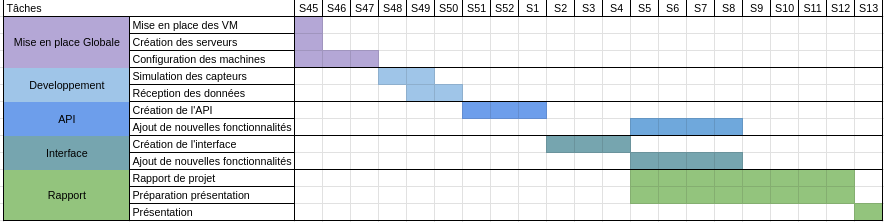
\includegraphics[width=1\textwidth]{ressources/img/Gantt/diagrammePrevisionnel}
		\caption{Diagramme de Gantt \textbf{Prévisionnel}}
		\label{fig:GanttPrevisionnel}
	\end{figure}
		\begin{figure}[h!]
		\centering
		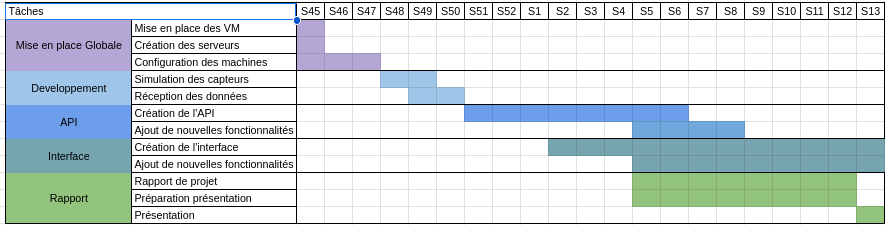
\includegraphics[width=1\textwidth]{ressources/img/Gantt/diagrammeReel}
		\caption{Diagramme de Gantt \textbf{réel}}
		\label{fig:GanttReel}
	\end{figure}
	
	\chapter{État de l'Art}
	\section{Technologies existantes}
	\section{Solutions alternatives et justification des choix}
	
	\chapter{Conception et Implémentation}
	
	\section{Infrastructure et Environnement de Développement}
	Cette section détaille l'ensemble de l’infrastructure mise en place, depuis la simulation logicielle d'une maison connectée jusqu'à l'infrastructure serveur dédiée. Cette dernière assure la \textbf{réception}, le \textbf{traitement} ainsi que le \textbf{stockage} sécurisé des données issues des différents capteurs IoT simulés. Nous présenterons les diverses technologies utilisées au sein de l'infrastructure, ainsi que la façon dont elles ont été intégrées afin de garantir une cohérence globale avec les objectifs initiales du projet.\\
	Ce projet a été réalisé en \textbf{local}, sous la forme d'une \textbf{simulation globale}. Le serveur utilisé repose sur une machine virtuelle exécutant \textbf{Ubuntu Server}, configurée localement via \textbf{un accès réseau en mode pont}. Cette configuration permet au serveur d'obtenir une adresse IP dédiée sur le même réseau local que la machine hôte, facilitant ainsi une connectivité réseau directe et simplifiée avec la maison connectée simulée. Dans ce contexte, notre simulation considère que le serveur et l’émetteur sont présents au sein du même réseau local, en l'absence de solution cloud externe.\\
	Nous verrons que le serveur joue un rôle centrale au sein de cette infrastructure. En effet, il héberge l'ensemble des services essentiels au fonctionnement de la solution réceptrice: Le \textbf{broker MQTT}, l'\textbf{API REST} développée sous Laravel, ainsi que l'ensemble des bases de données qu'elles soient à\textbf{ séries temporelles ou relationnelles}.\\
	Concernant l'infrastructure émettrice, afin de simuler les équipement IOTs de la \textbf{maison connectée}, nous avons utilisé le\textbf{ language Python} du fait de la disponibilité étendue des bibliothèques réseau faciles à implémenter, facilitant ainsi la mise en ouvre rapide et fiable de la simulation. \\
	Dans les sous-sections suivantes, nous détaillerons la mise en place précise de chacun des composants techniques essentiels à la réalisation de nos objectifs.
		\begin{figure}[h!]
		\centering
		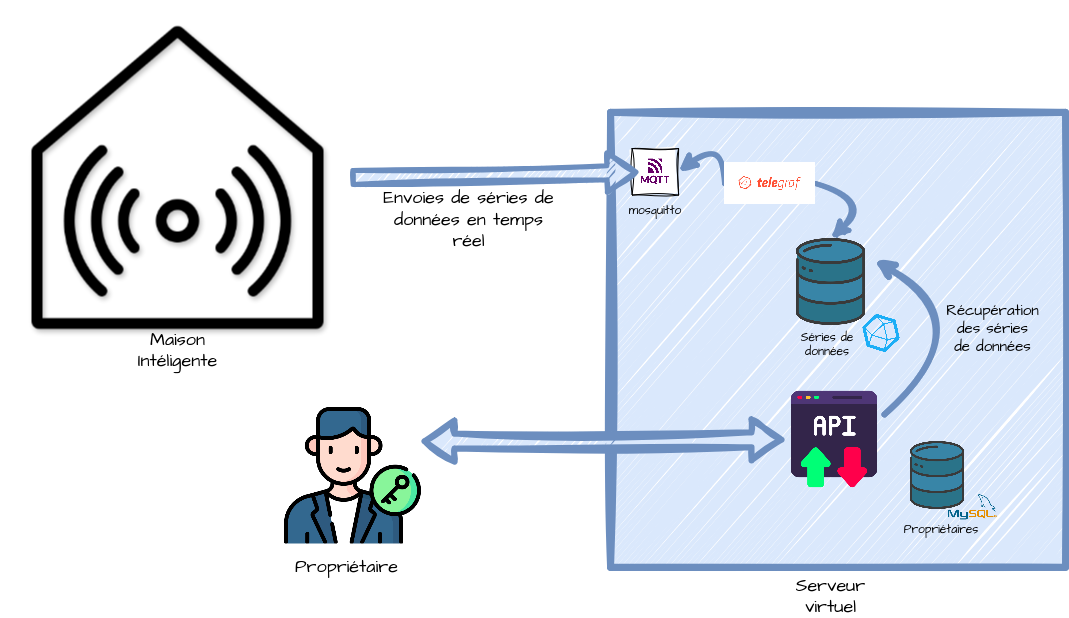
\includegraphics[width=0.5\textwidth]{ressources/img/shémas/shemaInfras.png}
		\caption{Architecture de l'infrastructure fonctionnelle}
		\label{fig:archiInfra}
	\end{figure}
	
	Le schéma ci-dessus décrit l'infrastructure globale mis en place décrit au sein de la section.
	
	
 
	\subsection{Simulation du serveur et architecture réseau}
	\subsubsection{Déploiement d'un Broker MQTT sécurisé}
	
	Afin de garantir une transmission en temps réel des données IOTs entre la maison connectée et le serveur, nous avons trouver plus judicieux de choisir le protocole \textbf{MQTT}.\\
	\textbf{MQTT} est un protocole de messagerie léger basé sur le modèle \textbf{publish/subscribe}, initialement concu pour des environnements où la bande passante est limitée et latence faible. MQTT est dans notre contexte parfaitement adapté, en effet, le protocole a initialement été concu afin d'être adapté aux applications IoTs, grâce à sa faible consommation de ressources, sa simplicité d'implémentation et son support pour des communications asynchrones et pouvant être sécurisées par le biais de la technologie \textbf{SSL/TLS}.\\\\
	Il est important de savoir que MQTT repose sur trois éléments fondamentaux:
	\begin{itemize}
		\item \textbf{Le Broker (serveur de message):} Element central de l'architecture MQTT agissant comme un relais entre les clients acheminant les messages publiés et les abonnés appropriés. Il en existe une variété, dans le cadre de notre projet, nous avons choisit d'utiliser \textbf{Mosquitto}.
		
		\item \textbf{Les Topics (Sujets de message):} Il s'agit d'une chaîne hierarchique permettant d'identifier une catégorie de message, leur format est composé de "/" permettant de séparrer les sous-topics. Dans le cadre de notre projet nous avons justement exploiter ce système de chaîne hiérarchique afin d'organiser d'une manière précise l'ensemble des types d'\textbf{iots} situés aux différentes salles des divers \textbf{maisons} des différents \textbf{propriétaires}. 
		
		\item \textbf{Les clients (publishers et subscribers):} MQTT fait la distinction entre deux types de clients: 
		\begin{itemize}
			\item \textbf{Les pusblishers (éditeurs)}, ceux qui envoient des messages à un topic spécifiques, sans se soucier du destinataire, il s'agit dans le cadre de notre projet, de la \textbf{maison connectée} qui envoies des series de données aux différents topics correspondant. 
			
			\item \textbf{Les subscribers (abonné)} ceux qui écoutent au sein d'un topic et reçoit les messages spécifiques correspondant, dans notre cas, il s'agit des \textbf{propriétaires} des maisons.
		\end{itemize}
	\end{itemize}
	\vspace{0.5cm}
	Tels qu'expliquait, nous avons choisis de déployer \textbf{Mosquitto} au sein du serveur. Malgré le fait qu'il existe d'autres solution tels que \textbf{HiveMQT}, \textbf{EMQX} ou \textbf{RabbitMQ MQTT}, pouvant faire office de \textbf{broker}, nous avons choisit \textbf{Mosquitto}, du fait qu'il est conçu pour être \textbf{ultra-lêger}, consommer \textbf{très peu de mémoire et de CPU même sous forte charge}, et convenir aussi bien \textbf{aux petits réseaux IoT qu'aux grandes infrastructures}.\\
	De plus, \textbf{Mosquitto} permet une installation assez rapide de son service, et la configuration s'effectue via un fichier \textbf{mosquitto.conf}. Enfin, il supporte des fonctionnalités de sécurité avancé que nous avons mit en place au sein de notre serveur, tels que le support \textbf{TLS/SSL} afin de chiffrer les communications.\\
	Pour sécuriser les connexions et assurer l'authenticité des communications, nous avons implémenté MQTT sécurisé (MQTTs) basé sur SSL/TLS. Nous avons utilisé l’outil \textbf{OpenSSL} pour créer une autorité de certification interne \textbf{CA} ainsi que pour \textbf{générer et signer automatiquement} des certificats clients \textbf{client.crt} et leurs clés privées associées \textbf{client.key}. Chaque maison simulée dispose donc de trois certificats essentiels pour établir une connexion sécurisée.\\\\
	Voici ainsi l'architecture de sécurisation de \textbf{Mosquitto}:
	\begin{itemize}
		 \item La création d'une Autorité de Certification (CA) dédiée pour la \textbf{génération et la signature des certificats}.
		\item L'utilisation de certificats clients signés (certificat client et clé privée) pour chaque maison voulant envoyer des données au sein d'un serveur.
		\item L'utilisation du protocole MQTTs, permettant une \textbf{authentification mutuelle} et un chiffrement systématique des communications, empêchant ainsi toute interception ou injection malveillante de données.
	\end{itemize}
	
	\vspace{1cm}
	
	Afin de faciliter la compréhension de la sécurisation de Mosquitto, et l'intégration du protocole MQTTs au sein de l'architecture, voici un schéma explicatif: 
	\newpage
	\begin{figure}[h!]
		\centering
		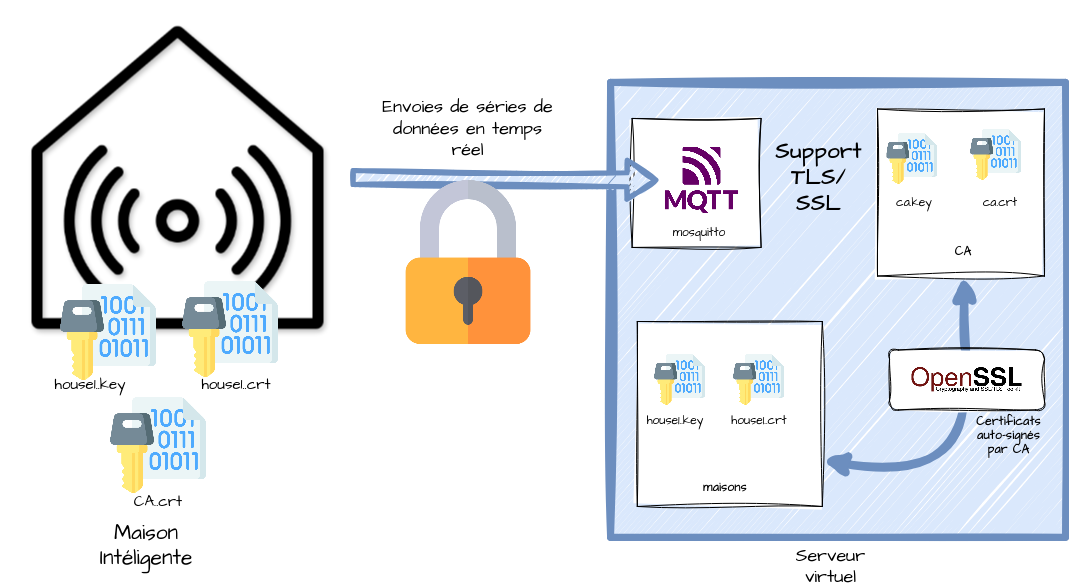
\includegraphics[width=0.5\textwidth]{ressources/img/shémas/shemaEmissionSSL.drawio.png}
		\caption{Sécurisation de mosquitto}
		\label{fig:secuMosquitto}
	\end{figure}
	
	Afin de vérifier le fonctionnement des certificats ainsi que l'envoi de données au sein du broker mosquitto du serveur virtuel, nous avons à ce moment là tester avec les commandes \textbf{mosquitto\_pub côté client} et les \textbf{logs temps réel côté serveur}\footnote{Au sein de la configuration de mosquitto, nous avons définit un chemin de log accessible en temps réel via la commande linux \textbf{tail -f /var/log/mosquitto/mosquitto.log}}.\\\\ Ainsi, après génération et auto-signature des certificats, les figures ci-dessous montrent ce qu'il se passe lorsque l'authentification est valide c'est à dire lorsque le \textbf{client.key} et le \textbf{client.crt} correspondent bien, et lorsque ces derniers sont invalides:
	
	\begin{figure}[h!]
		\centering
		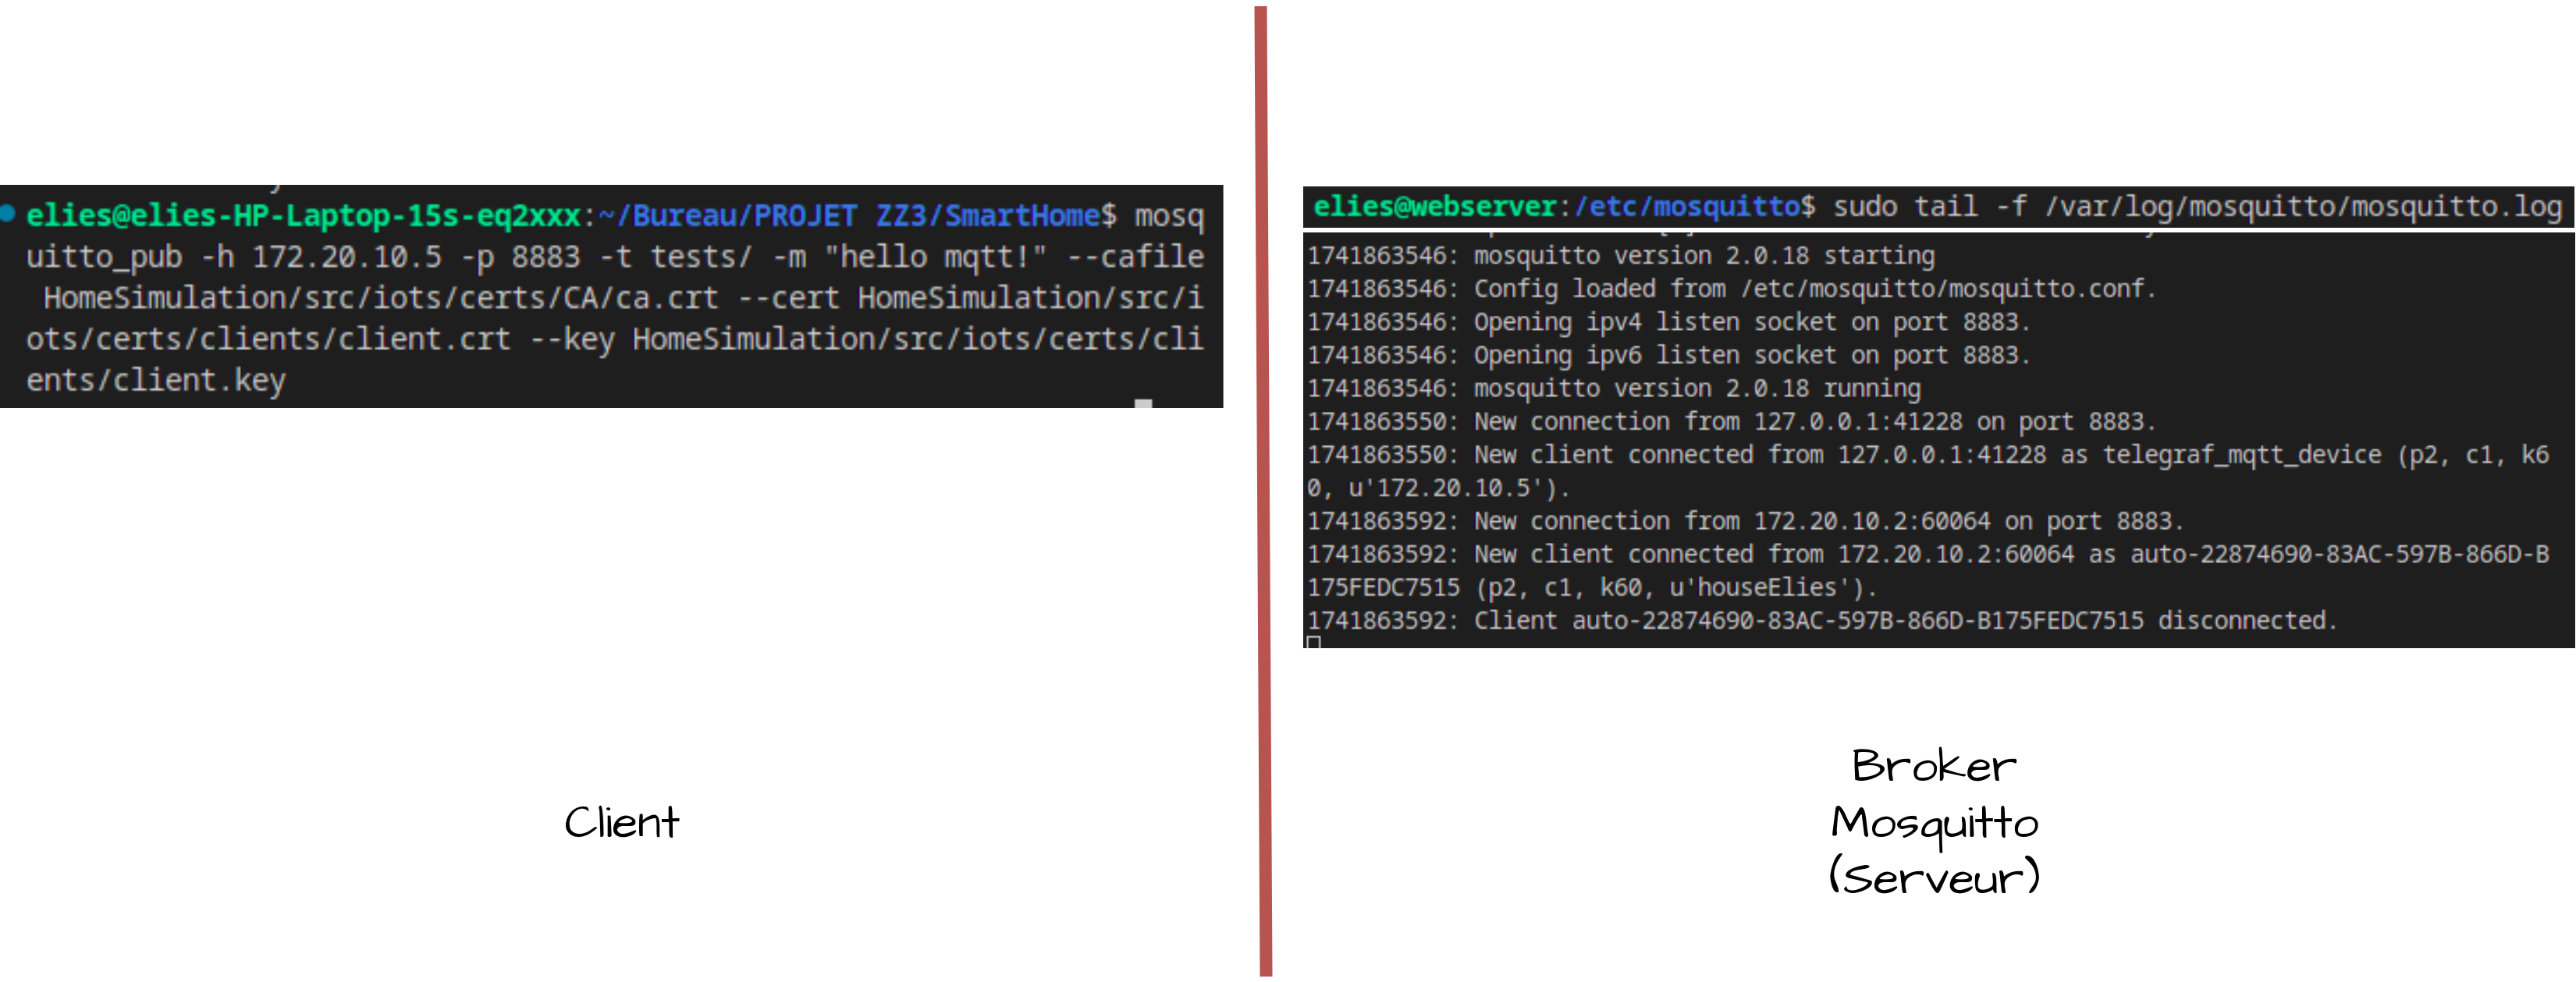
\includegraphics[width=1\textwidth]{ressources/img/preuves/emissionReceptionMosquittoValide.drawio}
		\caption{Authentification effectuée: Émission et réception effectuée avec succès}
		\label{fig:mosquittoValide}
	\end{figure}
	Dans la figure ci-dessus, nous pouvons nous apercevoir par la capture d'écran du résultat du log instantané du broker que la connexion de l'emetteur, s'est correctement déroulée, et que ce client a été correctement authentifiée par le nom d'utilisateur \textbf{houseElies}. \newpage
	
	\begin{figure}[h!]
		\centering
		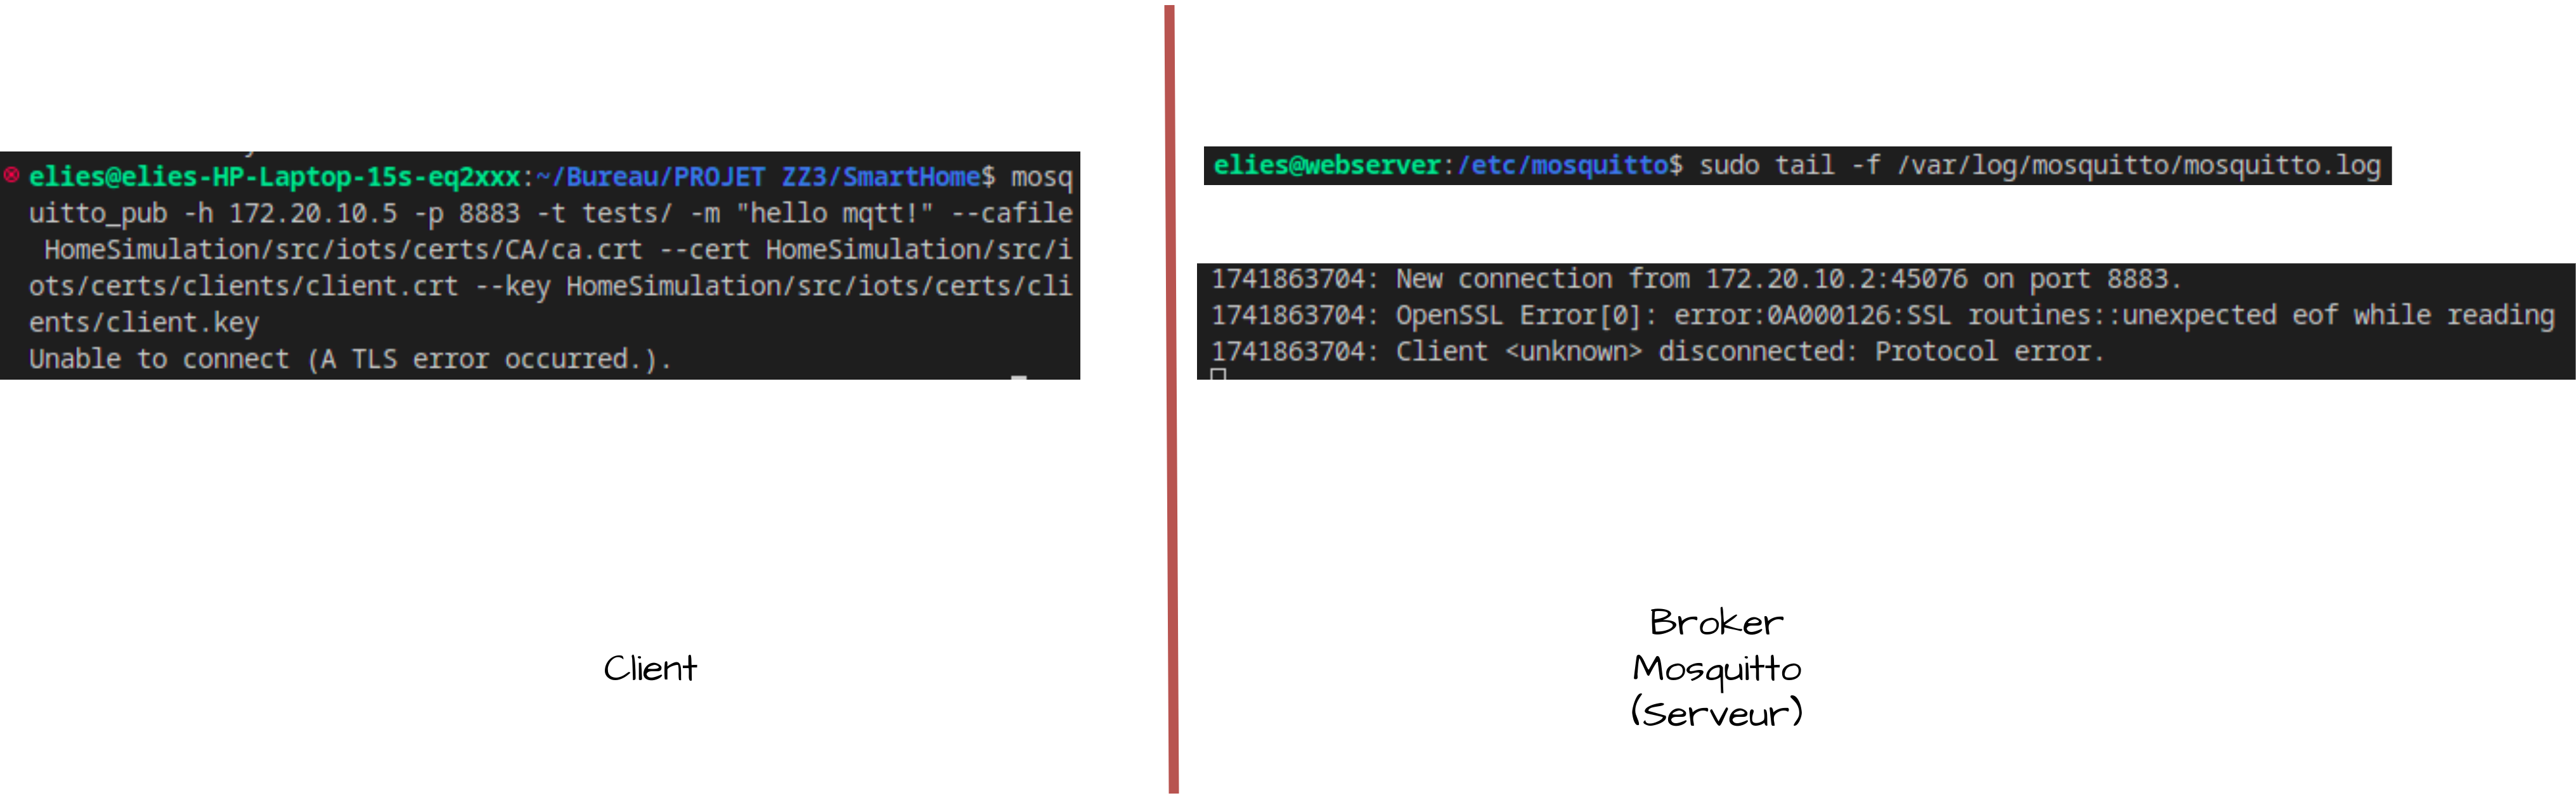
\includegraphics[width=1\textwidth]{ressources/img/preuves/emissionReceptionMosquittoInvalide.drawio}
		\caption{Authentification erronée: Émission et réception non fonctionnel}
		\label{fig:mosquittoInvalide}
	\end{figure}
	A la différence de la figure précédente, afin de prouver qu'il est nécéssaire de disposer de certificats clients valide, nous avons intentionnellement modifier la clès générée de manière à ce qu'elle soit erronée, nous pouvons ainsi constater qu'il y a une erreur lors de la connexion de l'emmeteur et que ce dernier n'est pas parvenue à publier, ni à être identifié par le broker.
	
	
	
	\subsubsection{Intégration d'une base de données à séries temporelles}
	
	L'emission de données sécurisé désormais possible au sein du serveur depuis une adresse IP distante, l'objectif du projet étant de permettre un accès à des données temps réel mais aussi des données capturés à une date donnée, il est nécéssaire de garantir un stockage de celles-ci.
	
	\subsubsection{Formalisation des données entre Mosquitto et InfluxDB}
	
	\subsection{Modélisation et Simulation d'une Maison Connectée}
	\subsubsection{Conception de l'architecture logicielle de la simulation}
	\subsubsection{Implémentation du protocole MQTTs}
	\subsubsection{Structuration et formalisation des données échangées}
	
	\section{Mise en place d'une API Web}
	\subsection{Architecture logicielle de l'API et choix technologiques}
	\subsection{Automatisation de l'authentification des maisons}
	\subsubsection{Mise en place d'une base de données MySQL}
	\subsubsection{Signature automatique des certificats}
	\subsection{Filtrage et récupération des données}
	\subsubsection{Communication avec InfluxDB API}
	
	\section{Surveillance des données avec une interface graphique}
	\subsection{Architecture logicielle de l'application SmartHouse Monitoring}
	\subsection{Intégration et communication avec l'API Web}
	\subsubsection{Authentification des maisons}
	\subsubsection{Affichage des données récupérées}
	
	\chapter{Résultats et Discussion}
	\section{Situation à la fin de l’étude}
	\section{Analyse des résultats obtenus}
	
	\chapter{Conclusion}
	\section{Conclusion du projet}
	\section{Limites et améliorations possibles}
	
	\appendix
	\chapter{Annexes}
	\section{Lexique}
	\section{Bibliographie}
	\section{Webographie}
	
	
	
		
	
	\nocite{*}
	\bibliographystyle{unsrt}
	\bibliography{references}
	
	\clearpage
	
	\printglossaries
	
	
\end{document}